\newpage
\section{Vector Calculus}

\subsection{Dot product}
\red{*This topic appears in 2 reference pages*} \\
\blue{Complete in reference page "vector and bases"} \\
\blue{Explained in reference page "vector identities"}

\subsection{Cross product}
\red{*This topic appears in 2 reference pages*} \\
\blue{Complete in reference page "vector and bases"} \\
\blue{Explained in reference page "vector identities"}

\subsection{Derivatives}
    \subsubsection{Cartesian}
    \blue{Complete in reference page "vector calculus"} \\
    \red{The example in Fig\ref{Fig:CartesianDerivatives} could be added:}
\begin{figure*}[!h]
\centering
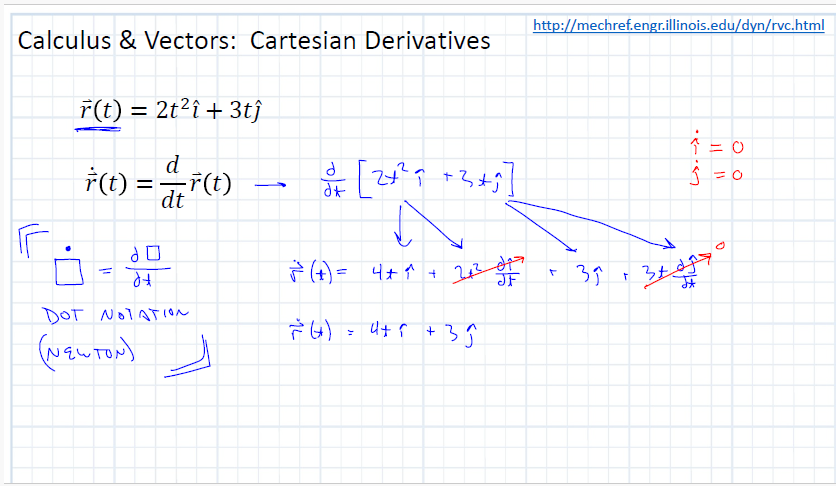
\includegraphics[width=0.9\textwidth]{VectorCalculusFigures/Cartesian Derivatives.png}
\vspace{-2mm}
\caption{\small Taken from L03-Notes, slide 6.}
\vspace{-3mm}
\label{Fig:CartesianDerivatives}
\end{figure*}
    
    \subsubsection{\red{Non-Cartesian: Polar basis}}
    \red{An example like in Fig\ref{Fig:Non-CartesianPolarBasis} could be added in "vector and bases"} 
\begin{figure*}[h!]
\centering
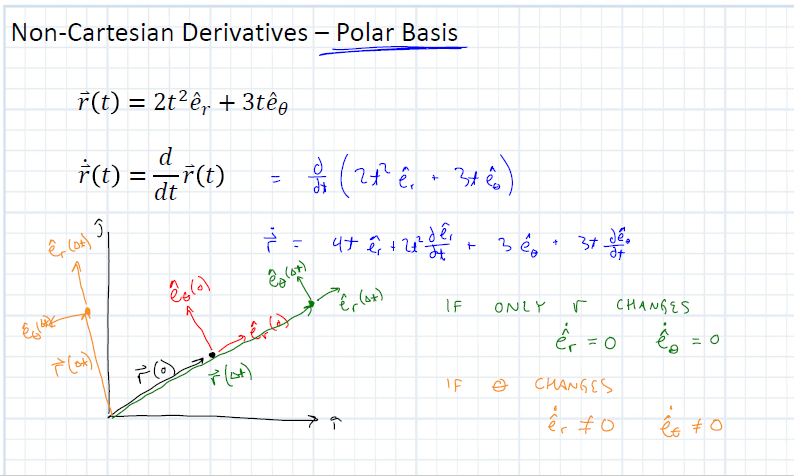
\includegraphics[width=0.9\textwidth]{VectorCalculusFigures/Non-Cartesian Polar Basis.png}
\vspace{-2mm}
\caption{\small Taken from L03-Notes, slide 7.}
\vspace{-3mm}
\label{Fig:Non-CartesianPolarBasis}
\end{figure*}
    
    \subsubsection{\red{Graphical estimation}}
        \red{The information in Fig \ref{Fig:GraphicalEstimation} could be included as a new section in "vector and bases"} 
\begin{figure*}[h!]
\centering
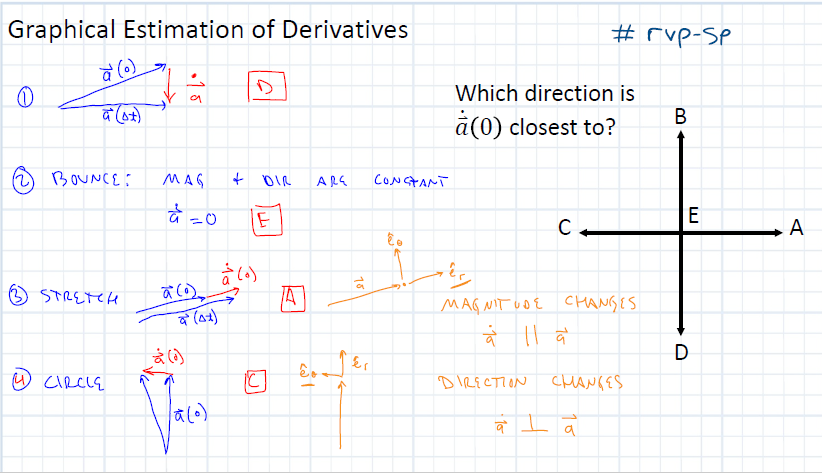
\includegraphics[width=0.9\textwidth]{VectorCalculusFigures/Graphical Estimation of Derivatives.png}
\vspace{-2mm}
\caption{\small Taken from L03-Notes, slide 8.}
\vspace{-3mm}
\label{Fig:GraphicalEstimation}
\end{figure*}

\subsection{Chain rule}
    \subsubsection{Scalars}
    \blue{Complete in "Vector Calculus"}
    \subsubsection{Second derivative}
    \blue{Complete in "vector Calculus"}
    
\subsection{\red{Integration}}
\red{Include summary of both Polar and Cartesian integration as in Fig \ref{fig:SummaryVecInt}}
\begin{figure}[h!]
    \centering 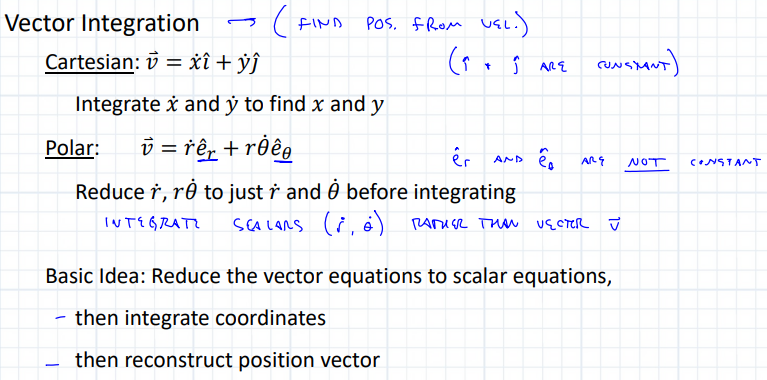
\includegraphics[width=0.8\textwidth]{VectorCalculusFigures/SummaryVectorIntegration.png}
    \caption{From L08-Notes, slide 6}
    \label{fig:SummaryVecInt}
\end{figure}
    \subsubsection{Cartesian basis}
    \blue{Complete in "Vector calculus"}
    \subsubsection{\red{Polar basis}}
    \red{Add the information in Fig \ref{fig:PolarIntegration}}
    
    \begin{figure}[h!]
        \centering 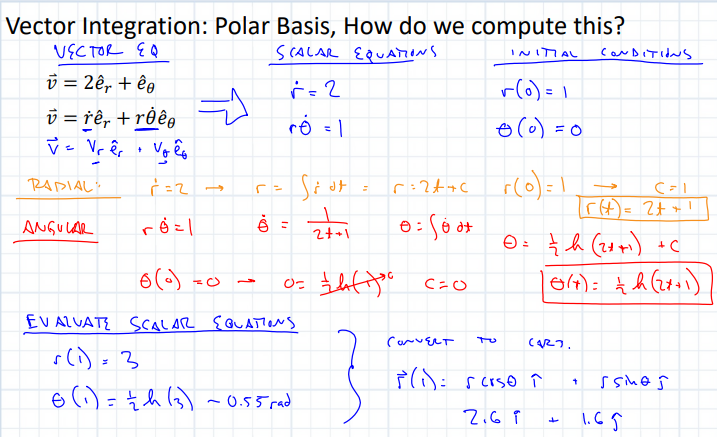
\includegraphics[width=0.8\textwidth]{VectorCalculusFigures/PolarIntegration.png}
        \caption{From L08-Notes, slide 5} \label{fig:PolarIntegration}
    \end{figure}

\subsection{\red{Solving equations}}
\red{Include step by step on how to solve vector equations as shown in Fig \ref{fig:SolvingEqnsSteps}}

\begin{figure}[h!]
    \centering 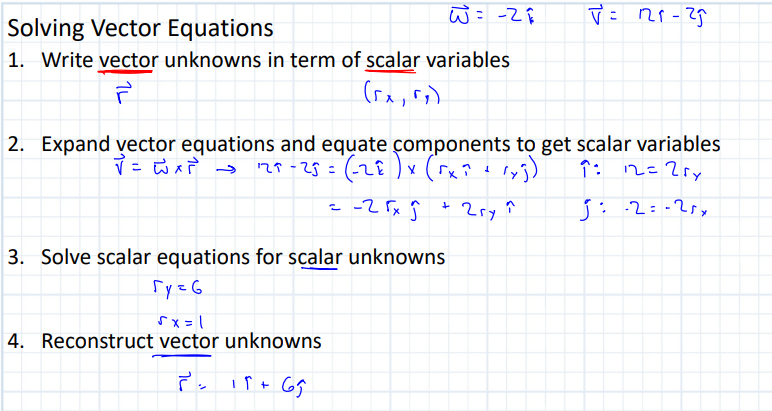
\includegraphics[width=0.8\textwidth]{VectorCalculusFigures/SolvingEqnsSteps.png}
    \caption{From L09-Notes, slide 10}
    \label{fig:SolvingEqnsSteps}
\end{figure}


Include examples as shown in Figs \ref{fig:SolvingEqns}, \ref{fig:SolvingEqns2} 

\begin{figure}[h!]
    \centering 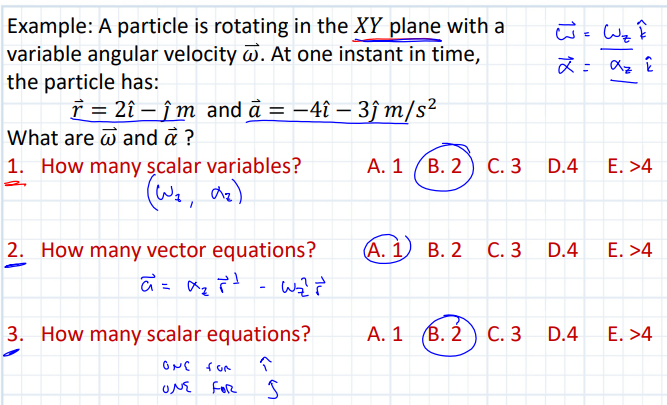
\includegraphics[width=0.8\textwidth]{VectorCalculusFigures/SolvingEqns.png}
    \caption{From L09-Notes, slide 9}
    \label{fig:SolvingEqns}
\end{figure}

\begin{figure}
    \centering 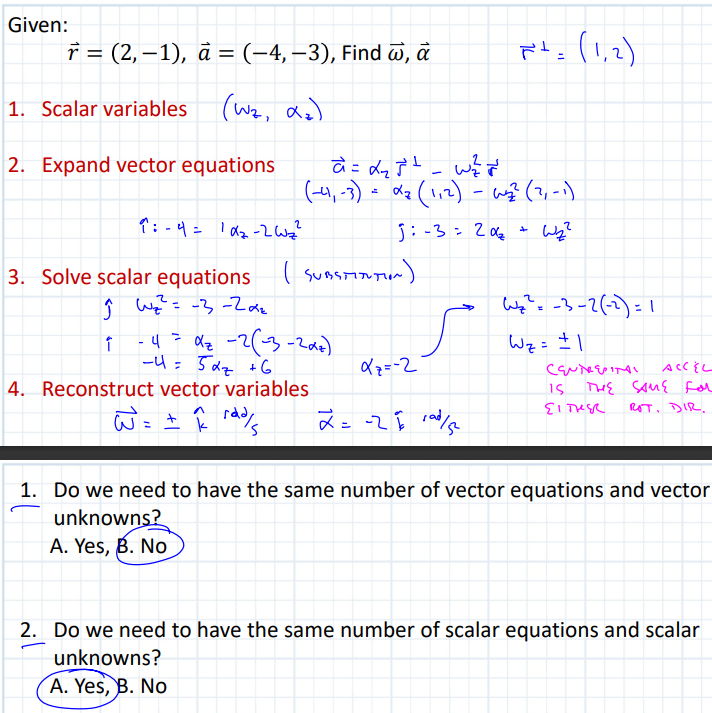
\includegraphics[width=0.8\textwidth]{VectorCalculusFigures/SolvingEqns2.png}
    \caption{From L10-Notes, slides 5-6}
    \label{fig:SolvingEqns2}
\end{figure}